%%%% Dokumentklassen %%%%

\documentclass[a4paper,11pt,fleqn,dvipsnames,twoside,openany]{memoir} 	% Openright åbner kapitler på højresider (openany begge)

\usepackage{wrapfig}
%%%% PACKAGES %%%%
%% Oversættelse og tegnsætning %%
\usepackage[utf8]{inputenc}					% Input-indkodning af tegnsæt (UTF8)
\usepackage[danish]{babel}					% Dokumentets sprog
\usepackage[T1]{fontenc}					    % Output-indkodning af tegnsæt (T1)
\usepackage{ragged2e,anyfontsize}			% Justering af elementer
\usepackage{fixltx2e}						% Retter forskellige fejl i LaTeX-kernen
\usepackage{eso-pic}		
\newcommand\BackgroundPic{%
\put(0,0){%
\parbox[b][\paperheight]{\paperwidth}{%
\vfill
\centering
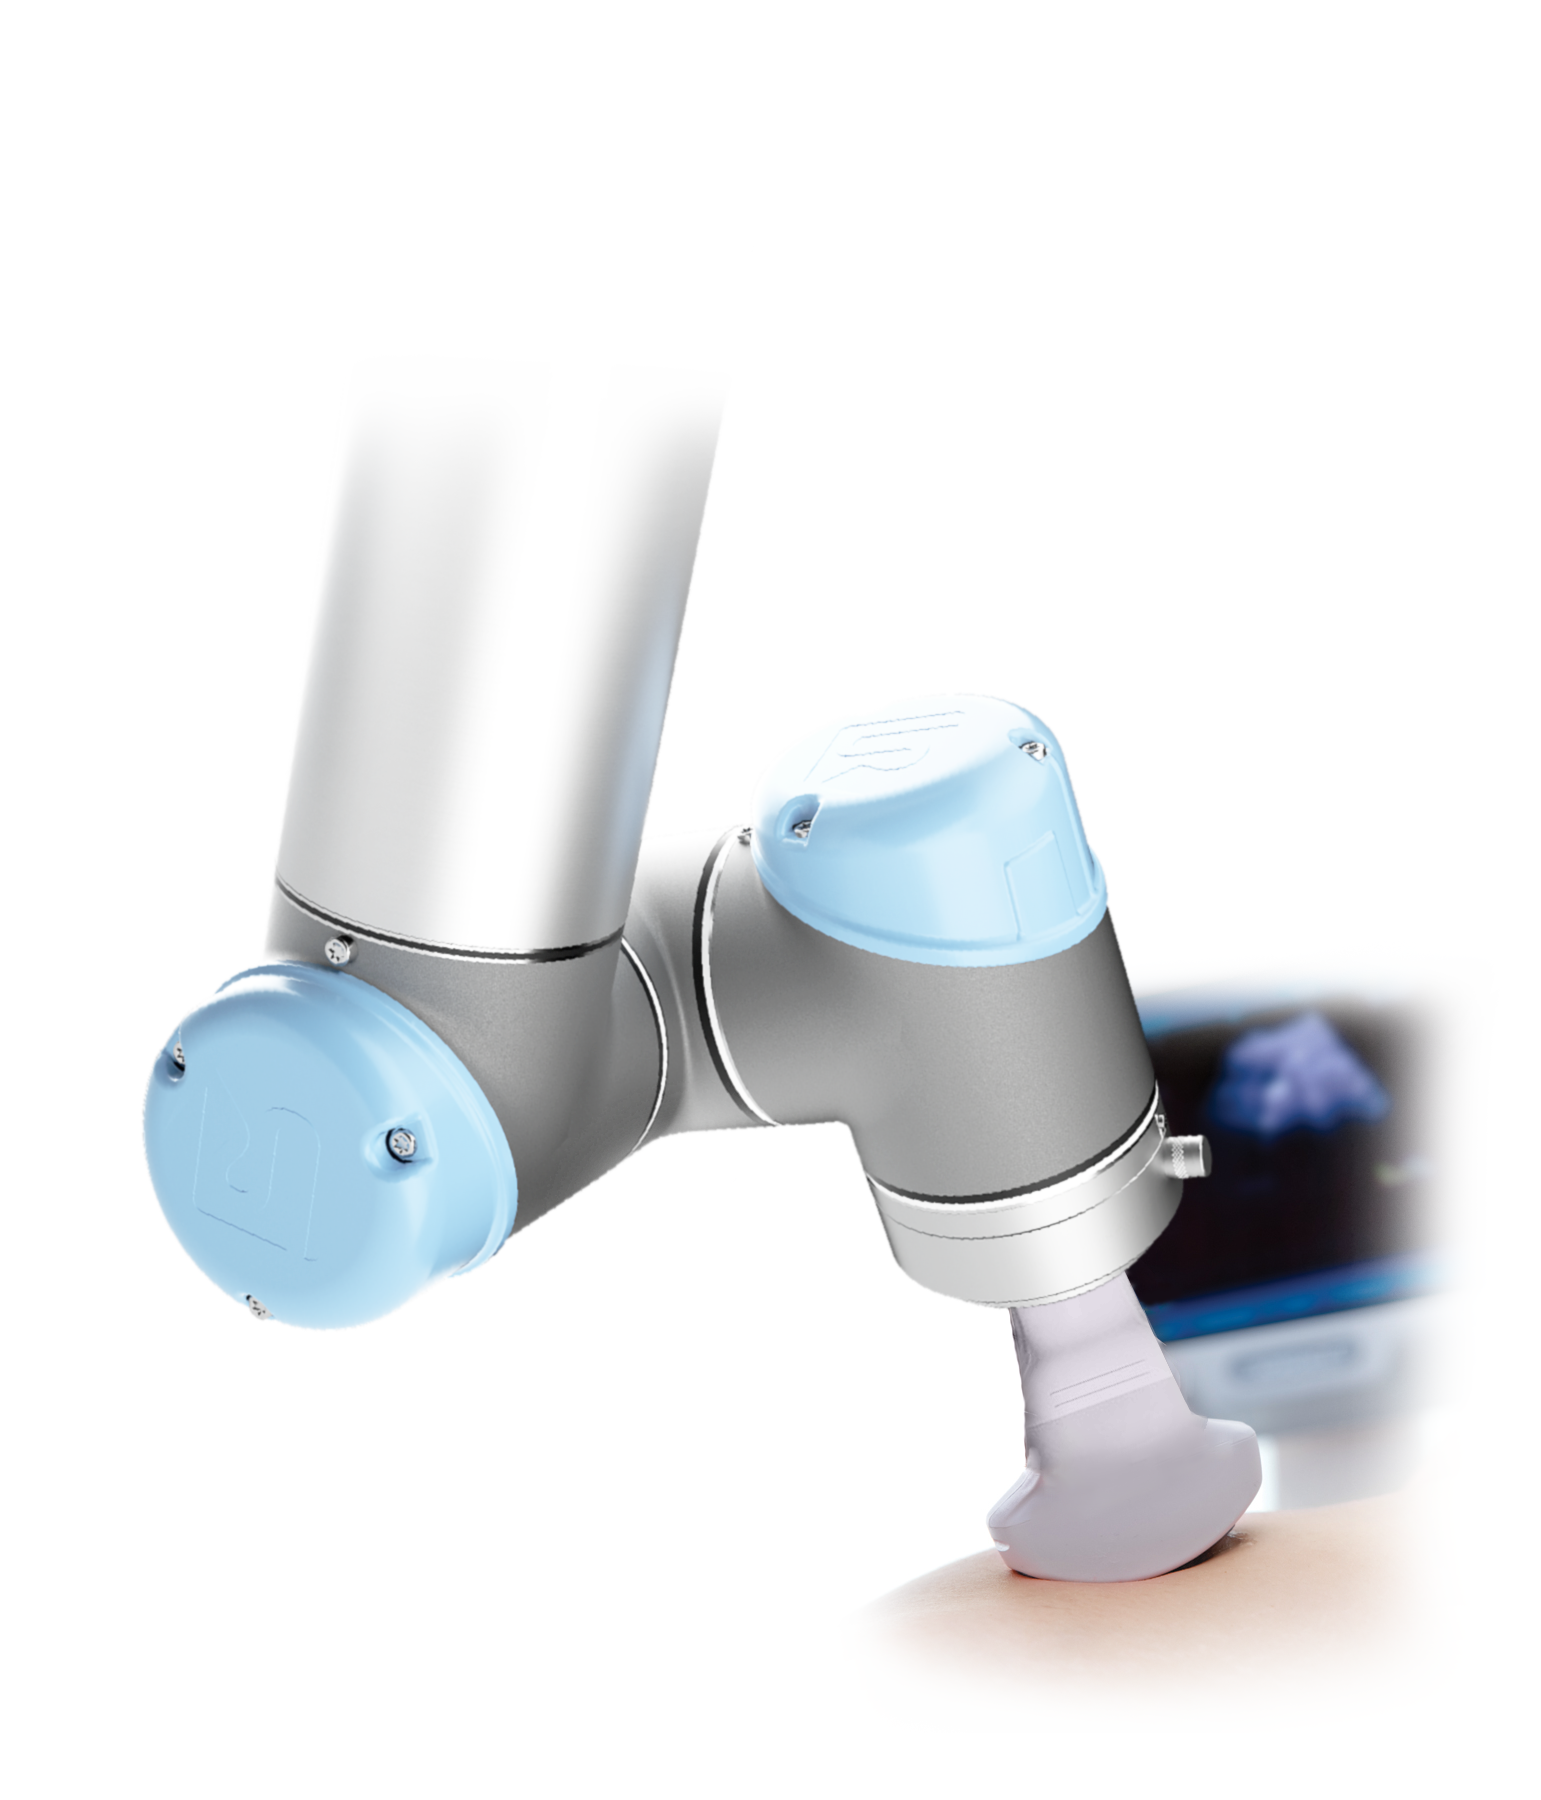
\includegraphics[width=\paperwidth,height=\paperheight,%
keepaspectratio]{figurer/forside.png}%
\vfill
}}}											
%% Figurer og tabeller (floats) %%
\usepackage{graphicx} 						% Håndtering af eksterne billeder (JPG, PNG, EPS, PDF)
\usepackage{multicol}         	            	% Muliggør output i spalter
\usepackage{rotating}						% Rotation af tekst med \begin{sideways}...\end{sideways}
\usepackage{xcolor}							% Definer farver med \definecolor. Se mere: http://en.wikibooks.org/wiki/LaTeX/Colors
\usepackage{flafter}						% Sørger for at floats ikke optræder i teksten før deres reference
\let\newfloat\relax 						% Justering mellem float-pakken og memoir
\usepackage{float}							% Muliggør eksakt placering af floats, f.eks. \begin{figure}[H]

%% Matematik mm. %%
\usepackage{amsmath,amssymb,stmaryrd} 		% Avancerede matematik-udvidelser
\usepackage{mathtools}						% Andre matematik- og tegnudvidelser
\usepackage{textcomp}                 		% Symbol-udvidelser (fx promille-tegn med \textperthousand)
\usepackage{rsphrase}						% Kemi-pakke til RS-saetninger, fx \rsphrase{R1}
\usepackage[version=3]{mhchem} 				% Kemi-pakke til flot og let notation af formler, f.eks. \ce{Fe2O3}
\usepackage{siunitx}						% Flot og konsistent præsentation af tal og enheder med \si{enhed} og \SI{tal}{enhed}
\sisetup{output-decimal-marker = {,}}		% Opsætning af \SI (DE for komma som decimalseparator) 
\usepackage{pdflscape}
\usepackage{afterpage}
%% Referencer og kilder %%
\usepackage[danish]{varioref}				% Muliggør bl.a. krydshenvisninger med sidetal (\vref)
\usepackage{natbib}							% Udvidelse med naturvidenskabelige citationsmodeller
\usepackage{xr}							    % Referencer til eksternt dokument med \externaldocument{<NAVN>}

%% Misc. %%
\usepackage{listings}						% Placer kildekode i dokumentet med \begin{lstlisting}...\end{lstlisting}
\usepackage{lipsum}							% Dummy text \lipsum[..]
\usepackage[shortlabels]{enumitem}			% Muliggør enkelt konfiguration af lister
\usepackage{pdfpages}						% Gør det muligt at inkludere pdf-dokumenter med kommandoen \includepdf[pages={x-y}]{fil.pdf}	
\pdfoptionpdfminorversion=6					% Muliggør inkludering af pdf-dokumenter, af version 1.6 og højere
\pretolerance=2500 							% Justering af afstand mellem ord (højt tal, mindre orddeling og mere luft mellem ord)	
\usepackage{hyperref}
%%%% CUSTOM SETTINGS %%%%
%% Marginer %%
\setlrmarginsandblock{3.5cm}{2.5cm}{*}		% \setlrmarginsandblock{Indbinding}{Kant}{Ratio}
\setulmarginsandblock{2.5cm}{3.0cm}{*}		% \setulmarginsandblock{Top}{Bund}{Ratio}
\checkandfixthelayout 						% Oversætter værdier til brug for andre pakker

%% Afsnitsformatering %%
\setlength{\parindent}{0mm}           		% Størrelse af indryk
\setlength{\parskip}{3mm}          			% Afstand mellem afsnit ved brug af double Enter
\linespread{1,1}							% Linjeafstand

%% Indholdsfortegnelse %%
\setsecnumdepth{subsection}		 			% Dybden af nummererede overskrifter (part/chapter/section/subsection)
\maxsecnumdepth{subsection}					% Dokumentklassens grænse for nummereringsdybde
\settocdepth{subsection} 					% Dybden af indholdsfortegnelsen
		
%% Opsætning af listings %%
\definecolor{commentGreen}{RGB}{34,139,24}
\definecolor{stringPurple}{RGB}{208,76,239}

\lstset{language=Matlab,					    % Sprog
	basicstyle=\ttfamily\scriptsize,		    % Opsætning af teksten
	keywords={for,if,while,else,elseif,		% Nøgleord at fremhæve
			  end,break,return,case,
			  switch,function},
	keywordstyle=\color{blue},				% Opsætning af nøgleord
	commentstyle=\color{commentGreen},		% Opsætning af kommentarer
	stringstyle=\color{stringPurple},		% Opsætning af strenge
	showstringspaces=false,					% Mellemrum i strenge enten vist eller blanke
	numbers=left, numberstyle=\tiny,		    % Linjenumre
	extendedchars=true, 					    % Tillader specielle karakterer
	columns=flexible,						% Kolonnejustering
	breaklines, breakatwhitespace=true,		% Bryd lange linjer
}

%% Navngivning %%
\addto\captionsdanish{
	\renewcommand\appendixname{Appendiks}
	\renewcommand\contentsname{Indholdsfortegnelse}	
	\renewcommand\appendixpagename{Appendiks}
	\renewcommand\appendixtocname{Appendiks}
	\renewcommand\cftchaptername{\chaptername~}		% Skriver "Kapitel" foran kapitlerne i indholdsfortegnelsen
	\renewcommand\cftappendixname{\appendixname~}	% Skriver "Appendiks" foran appendiks i indholdsfortegnelsen
}

%% Kapiteludssende %%
\definecolor{numbercolor}{gray}{0.7}		            % Definerer en farve til brug til kapiteludseende
\newif\ifchapternonum

\makechapterstyle{jenor}{					        % Definerer kapiteludseende frem til ...
  \renewcommand\beforechapskip{0pt}
  \renewcommand\printchaptername{}
  \renewcommand\printchapternum{}
  \renewcommand\printchapternonum{\chapternonumtrue}
  \renewcommand\chaptitlefont{\fontfamily{pbk}\fontseries{db}\fontshape{n}\fontsize{25}{35}\selectfont\raggedleft}
  \renewcommand\chapnumfont{\fontfamily{pbk}\fontseries{m}\fontshape{n}\fontsize{1in}{0in}\selectfont\color{numbercolor}}
  \renewcommand\printchaptertitle[1]{%
    \noindent
    \ifchapternonum
    \begin{tabularx}{\textwidth}{X}
    {\let\\\newline\chaptitlefont ##1\par} 
    \end{tabularx}
    \par\vskip-2.5mm\hrule
    \else
    \begin{tabularx}{\textwidth}{Xl}
    {\parbox[b]{\linewidth}{\chaptitlefont ##1}} & \raisebox{-15pt}{\chapnumfont \thechapter}
    \end{tabularx}
    \par\vskip2mm\hrule
    \fi
  }
}											        % ... her

\chapterstyle{jenor}						        % Valg af kapiteludseende - Google 'memoir chapter styles' for alternativer

%% Sidehoved %%

\makepagestyle{AAU}							        % Definerer sidehoved og sidefod udseende frem til ...
\makepsmarks{AAU}{%
	\createmark{chapter}{left}{shownumber}{}{. \ }
	\createmark{section}{right}{shownumber}{}{. \ }
	\createplainmark{toc}{both}{\contentsname}
	\createplainmark{lof}{both}{\listfigurename}
	\createplainmark{lot}{both}{\listtablename}
	\createplainmark{bib}{both}{\bibname}
	\createplainmark{index}{both}{\indexname}
	\createplainmark{glossary}{both}{\glossaryname}
}
\nouppercaseheads									% Ingen Caps ønskes

\makeevenhead{AAU}{\small BAC7 Automatisk Ultralydsscanner}{}{\leftmark}	% Definerer lige siders sidehoved (\makeevenhead{Navn}{Venstre}{Center}{Hoejre})
\makeoddhead{AAU}{\rightmark}{}{\small ASE}		            % Definerer ulige siders sidehoved (\makeoddhead{Navn}{Venstre}{Center}{Højre})
\makeevenfoot{AAU}{\small \thepage}{}{}						% Definerer lige siders sidefod (\makeevenfoot{Navn}{Venstre}{Center}{Højre})
\makeoddfoot{AAU}{}{}{\small \thepage}						% Definerer ulige siders sidefod (\makeoddfoot{Navn}{Venstre}{Center}{Højre})

\copypagestyle{AAUchap}{AAU}							% Sidehoved for kapitelsider defineres som standardsider, men med blank sidehoved
\makeoddhead{AAUchap}{}{}{}
\makeevenhead{AAUchap}{}{}{}
\makeheadrule{AAUchap}{\textwidth}{0pt}
\aliaspagestyle{chapter}{AAUchap}					% Den ny style vælges til at gælde for chapters
													% ... her
															
\pagestyle{AAU}										% Valg af sidehoved og sidefod


%%%% CUSTOM COMMANDS %%%%

%% Billede hack %%
\newcommand{\figur}[4]{
		\begin{figure}[H] \centering
			\includegraphics[width=#1\textwidth]{billeder/#2}
			\caption{#3}\label{#4}
		\end{figure} 
}

%% Specielle tegn %%
\newcommand{\decC}{^{\circ}\text{C}}
\newcommand{\dec}{^{\circ}}
\newcommand{\m}{\cdot}


%%%% ORDDELING %%%%

\hyphenation{mmHg}    %% Her kan defineres ordelingen for specifikke ord med "-". De forskellige ord adskilles med mellemrum. Fx \hyphenation{er-hvervs-liv-et Himmelstrup ka-kao}. I de fleste tilfælde kan LaTeX selv stå for det.

%%%% Tilføjelser af min preample %%%%

% Booktabs:
% The booktabs package is needed for better looking tables. 
\usepackage{booktabs}

% Caption:
% For better looking captions. See caption documentation on how to change the format of the captions.
\usepackage[hang, font={small, it}]{caption}

% Hyperref:
% This package makes all references within your document clickable. By default, these references will become boxed and colored. This is turned back to normal with the \hypersetup command below.
\usepackage{hyperref}
	\hypersetup{colorlinks=false,pdfborder=0 0 0}

% Cleveref:
% This package automatically detects the type of reference (equation, table, etc.) when the \cref{} command is used. It then adds a word in front of the reference, i.e. Fig. in front of a reference to a figure. With the \crefname{}{}{} command, these words may be changed.
\usepackage{cleveref}
	\crefname{equation}{formel}{formler}
	\crefname{figure}{figur}{figurer}	
	\crefname{table}{tabel}{tabeller}
	\crefname{section}{afsnit}{afsnit}
	\crefname{chapter}{kapitel}{kapitler}

% Mine tilføjelser:
\usepackage{nameref}                      %% Bruges til at kunne referere til kapitler og afsnits navne.
\usepackage{units}                        %% Bruges til at gøre fx 1/2 samlet med: \nicefrac{1}{2}.
\usepackage{tabu, longtable}              %% Bruges til tabeller.
\setlength{\tabulinesep}{2ex}             %% Definerer linjeafstand i tabeller.
\usepackage{enumerate}                    %% Bruges til lister.
\usepackage{tabto}                        %% Giver mulighed for TAB med fx \tabto{3em}.
\usepackage[hyphenbreaks]{breakurl}       %% Bruges til websiders url'er.
\renewcommand{\UrlFont}{                  %% Definerer url-font.
\small\ttfamily}                          %
\bibliographystyle{plain}                 %% Definere bibliografien. Ses til sidst i dokumentet i kapitlet Litteratur.
\raggedbottom
\usepackage{todonotes}
\presetkeys{todonotes}{inline}{}
\externaldocument[D-]{Dokumentation}
\externaldocument{Bilagsliste}

\begin{document}

\begin{titlingpage}
\begin{center}

~ \\[3cm]


\includegraphics[width=0.6\textwidth]{figurer/ASE}~\\[1cm]

\textsc{\LARGE Aarhus University School of Engineering}\\[1.5cm]

\textsc{\Large Sundhedsteknologi og Informations- og kommunikationsteknologi}\\
\textsc{\Large Bachelorprojekt}\\[0.5cm]
\textsc{\Large Dokumentation} \\[1cm]

\noindent\makebox[\linewidth]{\rule{\textwidth}{0.4pt}}\\
[0.5cm]{\Huge Automatisk Ultralydsscanner}
\noindent\makebox[\linewidth]{\rule{\textwidth}{0.4pt}}

\end{center}

Charlotte Søgaard Kristensen (201371015) \newline
Mathias Siig Nørregaard  (201270810)\newline		 
Marie Kirkegaard (201370526) \newline  

\textit{Vejleder} \newline
Associate Professor\\
Michael Alrøe\\
Aarhus University School of Engineering


\vfill

\begin{center}
{\large 16. december}
\end{center}

\end{titlingpage}
\cleardoublepage

		
\mainmatter
\tableofcontents 

% Her findes de nummererede kapitler modsat \frontmatter og \backmatter.
%\chapter{Forkortelser}

\begin{table}[htb]
\centering
\begin{tabular}{ | c | p{0.80\textwidth} | }
\hline
\textbf{Forkortelser} & \textbf{Forklaring} \\\hline
ASE & Aarhus School of Engineering \\\hline
BDD & Block Definition Diagram \\\hline
FURPS+ & Funkctionality, Usability, Reliability, Performance, Supportability and Ekstra \\\hline
GUI & Graphical User Interface, Grafisk brugergrænseflade \\\hline
IBD & Internal Block Diagram \\\hline
MDD & Medical Device Directive \\\hline
MoSCoW & Must, Should, Could and Would like \\\hline
QALY & Kvalitet justeret leveår  \\\hline
RCT & randomized controlled trial \\\hline
SysML & Systems Modeling Language \\\hline
UC & Use case \\\hline
UML & Unified Modeling Language \\\hline

\end{tabular}
\caption{Forkortelser}
\end{table}

\vspace{3cm}
\chapter{Versionshistorik}\label{Versionshistorik}

\begin{table}[htb]
\begin{tabular}{ | l | l | l | p{0.49\textwidth} | }
\hline
\textbf{Version} & \textbf{Dato} & \textbf{Ansvarlig} & \textbf{Beskrivelse} \\\hline
1.0 & 2016-11-01 & CSK & Første version af udviklingsdokuement med systembeskrivelse, bdd og ibd\\\hline
1.1 & 2016-11-03 & CSK & Sekvensdiagrammer tilføjet  \\\hline
1.2 & 2016-11-04 & CSK, MSK & Forklaringer til sekvens- og klassediagrammer \\\hline
\end{tabular}
\caption{Versionshistorik}
\end{table}
\chapter{Indledning}
\section{Baggrund}
Danmark vil i de kommende årtier få en voksende andel af ældre borgere, der vil lægge et større pres på velfærdssamfundet i Danmark. Det vil resultere i færre borgere i den arbejdsdygtige alder, da det ud fra en befolkningsfremskrivning til 2040 forventes, at andelen af personer på 65 år og derover vil udgøre omkring en fjerdedel af den samlede danske befolkning \cite{Befolk}. En sådan ændring i demografien vil betyde flere patienter med kroniske lidelser, som derved vil medføre øgede omkostninger for og pres på sundhedsvæsenet \citep{Pres}. Det er derfor nødvendigt, at se på optimerede løsninger til behandling og diagnosticering af sygdomme. 

I Danmark tilbydes alle kvinder i alderen 50 til 69 år en rutinemæssig mammografiscreening. Mammografiscreening foregår ved en røntgenundersøgelse, hvilket er billigt og effektiv \cite{Afsloring}. Metoden er dog ikke altid den mest hensigtsmæssige at anvende, da kirtelvæv og ondartede cancersvulster kan være svære at skelne fra hinanden på et røntgenbillede. Røntgenmetoden har derfor en begrænset undersøgelseseffekt ved kvinder med meget kirtelvæv. Til disse patienter suppleres røntgenbillederne med en ultralydsundersøgelse, som fortages af en radiolog \cite{Ultralyd}.

Ultralyds- og røntgenundersøgelser har hver sine fordele og kan derfor sjældent stå alene. Ultralyd har den største diagnosesikkerhed i kirtelvæv, hvor røntgen har den største diagnosesikkerhed i fedtvæv. Da brystet ofte er en kombination af de to vævstyper, supplerer disse to metoder hinanden godt \cite{Ultralyd}. 

Mammografi foretages i dag af enten en radiograf eller en røntgensygeplejerske, hvorefter røntgenbillederne bliver sendt videre til en radiolog. I fremtiden kunne det forestilles, at automatiserede ultralydsscanninger til screening for brystkræft kunne foretages med samme procedure, hvor ultralydsvideoclips efterfølgende sendes til lægen.

Dette bachelorprojekt går derfor ud på at lave et Proof of Concept, for af undersøge muligheden for automatiserede ultralydsscanninger til screening for brystkræft.
\newpage

\section{Problemformulering}
Med udgangspunkt i projektets baggrund og projektbeskrivelse, er der defineret følgende problemstillinger, som forsøges besvaret og belyst i dette bachelorprojekt. Se bilag \ref{Projektbeskrivelse} Projektbeskrivelse (ASE)

\textbf{Hvordan kan en automatiseret ultralydsscanner til screening for brystkræft udvikles samt hvilke økonomiske og produktsikkerhedsmæssige tiltag vil kunne realisere dette?}

\let\labelitemi\labelitemii
\begin{itemize}
\item Hvordan vil en automatiseret ultralydsscanning til screening for brystkræft kunne udvikles ved brug af robotarm og 3D kamera?
\item Hvilke omkostninger vil indførslen af en Automatisk Ultralydsscanner kunne give? 
\item Hvilke konsekvenser vil en tilføjelse af Automatisk Ultralydsscanner til screeningsprogrammet have?
\item Hvad kræves for at få Automatisk Ultralydsscanner CE-mærket? 
\end{itemize}

\chapter{Systemarkitektur}\label{Systemarkitektur}
Der er udarbejdet forskellige diagrammer på baggrund af de specificerede systemkrav.  Diagrammerne har til formål at dele systemet op i realiserbare dele for at vise arkitekturen for systemet. 

Arkitekturen beskriver den grundlæggende organisering af Automatisk Ultralydsscanner og opbygningen af dens tilhørende PC Applikation. Systemet er opbygget generisk, så man vil kunne udskifte komponenter som f.eks. Robotarm eller 3D kamera med en anden type eller model. Udskiftning af komponenter vil dog resultere i en anderledes implementering. Der er i diagrammerne designet ud fra, at 3D kamera er af typen Microsoft Kinect 2.0 og Robotarm er en UR10 robot. 

\section{Systemoversigt}
Systemet Automatisk Ultralydsscanner består af en PC applikation, en Ultralydsscanner, en Robotarm af typen Universal Robots UR10, et 3D kamera af typen Microsoft Kinect 2.0, samt et Access Point, af typen D-Link DAP-1160, til forbindelse mellem Robotarm og PC applikation. Der er fem aktører, Robotarm, Ultralydsscanner, 3D kamera, Operatør og Patient, som interagerer med PC Applikation.

Robotarm har en touch skærm, hvorpå Operatør manuelt kan flytte Robotarm, se Robotarms koordinator samt programmere Robotarm. Robotarm er forbundet via et ethernet kabel af typen RJ45 til et Access Point. PC Applikation er forbundet til Access Point med et kabel af samme type. 3D kamera er forbundet til PC Applikation via 3D kameras USB 3.0 kabel. Ultralydsscanner er en seperat enhed, som blot er fastgjort mekanisk på Robotarms yderste led, men indgår i det fulde system Automatisk Ultralydsscanner. Ultralydsscanner skal manuelt tændes og slukkes af Operatør.

For Automatisk Ultralydsscanner er der udarbejdet forskellige diagrammer, som har til formål at dele systemet op i blokke og vise integration mellem blokkene, samt forbindelser mellem aktører. Diagrammerne vil blive gennemgået nedenfor. 
\newpage

\subsection{Domænemodel}
Domænemodellen på Figur \ref{domain} viser forbindelserne mellem de forskellige aktører i systemet. 

\begin{figure}[H]
    \centering
    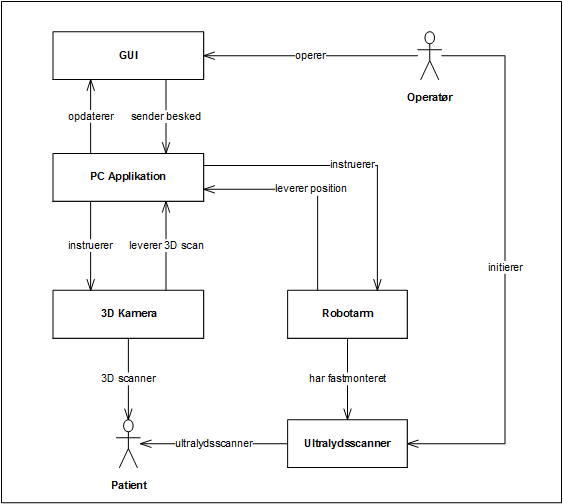
\includegraphics[width=0.7\textwidth]{figurer/d/Design/uml_domain}
    \caption{Domænemodel for Automatisk Ultralydsscanner}
    \label{domain}
\end{figure}

\subsection{Block Definition Diagram}
Block Definition Diagram Figur \ref{BDD} giver et overblik over Automatisk Ultralydsscanners komponenter, som et samlet system.
Her ses, at det er nødvendigt at have en computer med mus og skærm for at anvende PC Applikation.

\begin{figure}[H]
    \centering
    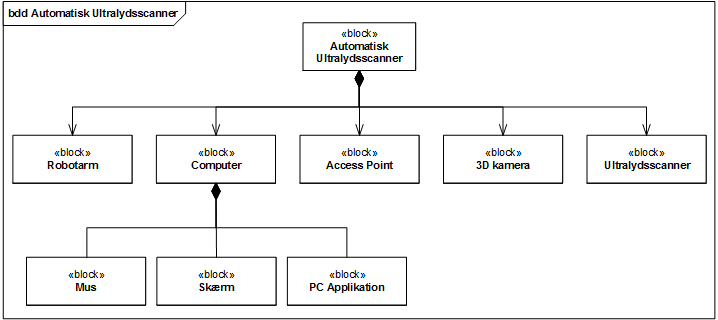
\includegraphics[width=1\textwidth]{figurer/d/Design/BDD}
    \caption{BDD for Automatisk Ultralydsscanner}
    \label{BDD}
\end{figure}
\newpage

\subsection{Internal Block Diagram}
Internal Block Diagram Figur \ref{IBD} viser flow af information mellem de forskellige blokke i Automatisk Ultralydsscanner.
Bemærk at Ultralydsscanner ikke er med, da den ikke interagerer med resten af Automatisk Ultralydsscanner, men blot er forbundet mekanisk til Robotarm.
Når 3D Scan menuen åbnes i PC Applikation, vil der være et konstant flow af dybdedata fra 3D kamera til PC Applikation.
Når PC Applikation startes, vil der være et flow af data frem og tilbage mellem Robotarm og PC Applikation, hvor Access Point agerer som mellemled. 
Forbindelsen mellem PC Applikation og Access Point, samt forbindelsen mellem Access Point og Robotarm er oprettet med ethernet-kabler af typen RJ45.
Forbindelsen mellem PC Applikation og 3D kamera er oprettet med 3D kameras USB 3.0 kabel. 

\begin{figure}[H]
    \centering
    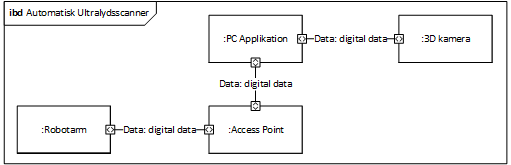
\includegraphics[width=1\textwidth]{figurer/d/Design/IBD}
    \caption{IBD for Automatisk Ultralydsscanner}
    \label{IBD}
\end{figure}

\section{Systemets grænseflader}
Systemet består af to grænseflader: Mellem PC Applikation og Kinect, og mellem PC Aplikation og UR10. Kommunikationen mellem PC Applikation og UR10 sker over modbus-protokollen, hvor kommunikationen mellem PC Applikation og Kinect er gennem Kinect's API.

\subsection{UR10}
Overførsel af data til UR10 sker gennem Transmission Control Protocol/IP-protokollen (TCP/IP). Til afsendelse af positur-værdier fra PC Applikation anvendes modbus-protokollen. Modbus-protokollen sørger for at skrive binære værdier på registre på UR10-controlleren. UR10 kører på URScripts, hvis den skal styres automatisk. UR10 har et script der i en uendelig løkke læser værdierne på registrene og instruerer UR10s Tool Center Point (TCP) til at flytte sig til en positur med en given acceleration og hastighed.

\subsubsection{TCP/IP}
PC Applikation skriver til UR10 over en TCP/IP forbindelse på en IP. Der anvendes to porte; port 502 for kommunikation over modbus-protokollen, og port 30002 for indlæsning af nuværende værdier.
Kommunikationen over port 502 er både read og write, hvor port 30002 kun er read. 
Bemærk, at forskellen  ligger i at de værdier der bliver overført på port 502 kun er til styring af UR10 på script-niveau, som fx den ønskede positur, hastighed og acceleration. Modsat, på port 30002, indhentes de nuværende tilstandsværdier som UR10 har, som fx posituren den reélt har, som ikke nødvendigvis er den samme som den sidste ønskede positur.
For at give et eksempel på hvordan dette foregår sekvensmæssigt:
PC Applikation sender en positur over port 502. Værdierne i denne positur indskrives på UR10s registre.
URScriptet aflæser disse værdier og instruerer UR10 i at flytte sit TCP til denne positur.
Efter noget tid vil den have nået denne positur. Der vil løbende kunne aflæses om UR10 har nået posituren på port 30002.

\textbf{Port 502}
Skriv tekst

\textbf{URScript}
Scriptet der kører på UR10 aflæser i alt 3 værdier:
Acceleration, hastighed og positur.
Positur består af værdierne X, Y og Z for position og RX, RY og RZ for rotation.
Positur-værdierne aflæses på registrene 135-140 og indsættes som properties i et 'pose' objekt.
Accelerationsværdien, hastighedsværdien samt pose-objektet gives som parameter til funktionen \textit{movel}.
UR10s TCP flyttes lineært i funktionen \textit{move1}. Tiden på acceleration og deceleration styres omvendt proportionalt af accelerationsværdien, mens den maksimale hastighed styres af hastighedsværdien.

\textbf{Port 30002}
Der er mulighed for at hive informationer om stort set alle robottens nuværende tilstande som fx software version, ledrotationshastighed, tryk feedback m.m. I implementeringen anvendes der kun TCPs rotation og position.

\subsection{Kinect}
Computeren er forbundet til 3D kamera via USB af typen Transcend PDU3 USB-adapter PCIe 2.0 USB 3.0 eller anden USB3.0 type, der er kompatible med Microsoft Kinect 2.0. 3D kamera har også et supplerende strømforsyningskabel.
For kommunikation med 3D kamera er der brugt Microsoft's Kinect API \cite{KinectAPI} .
Der er taget udgangspunkt i Fusion-delen \cite{KinectFusion} af API'et. Fordelen med dette API er at det kan gøre en masse arbejde - ulempen er at det ikke er generisk. Altså ville man ikke kunne bruge en anden sensor en Microsoft Kinect for Windows 2.0. API'et har en C\#-wrapper, og Microsoft har leveret kildekode til et projekt der gjorde nogenlunde det vi var interesserede i (se reference \cite{KinectFusionExplorer} for at få den nyeste version af dette.
Efter oprettelsen af forbindelse til Kinect sensoren er det muligt at 'lytte' på den og få de depth frames den kontinuerligt leverer. Se beskrivelsen af klassen KinectFusionizer underafsnittet \ref{ComputerVisionLibrary}  ComputerVisionLibrary. 

\newpage

\section{Softwarearkitektur}
PC Applikation er opdelt af forskellige moduler for at øge samhørigheden og nedsætte koblingen, hvilket er med til at sikre overskuelighed og gøre PC Applikation lettere at vedligeholde og genbruge. Modulerne er inddelt efter ansvarsområder angående præsentation til bruger, kommunikation til Robotarm, indhentning af 3D scan fra 3D kamera samt udregning af Robotarms sti til ultralydsscanning. Disse 4 moduler har fælles datastrukturer. For at undgå cykliske forbindelser, er disse datastrukturer tilføjet til deres eget modul. Figur \ref{Layers} viser referencen mellem modulerne. 

\begin{figure}[H]
    \centering
    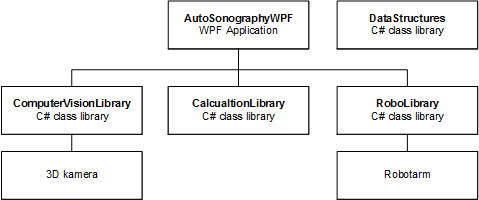
\includegraphics[width=0.75\textwidth]{figurer/d/Design/Layers}
    \caption{PC Applikations opdeling af moduler}
    \label{Layers}
\end{figure}


\begin{table}[htb]
\begin{tabular}{ | l | p{0.7\textwidth} | }
\hline
\textbf{Lag} & \textbf{Beskrivelse af ansvar} \\\hline
AutoSonographyWPF & Håndterer Operatørs interaktion med PC Applikation, hvor Operatør kan vælge 3D scan- eller ultralydsscan. Dette projekt virker som en grænseflade til resten af PC Applikation.\\\hline
ComputerVisionLibrary & Indhenter og afgrænser 3D scanning fra 3D kamera. \\\hline
CalculationLibrary & Sørger for at konvertere en 3D scanning til en sti af positurer som Robotarm kan gennemløbe. \\\hline
RoboLibrary & Muliggør at kommunikere med og instruere Robotarm.\\\hline
DataStructures & Indeholder forskellige data transfer objekter (DTO), der bruges gennem PC Applikation til at sende objekter mellem de forsellige moduler, samt udvidelsesmetoder til eksisterende .NET eller KinectAPI datastrukturer.\\\hline
\end{tabular}
\caption{Modulopdeling og ansvar}
\end{table}

\newpage
\subsection{Pakkediagram}
Pakkediagrammet figur \ref{Pakkediagram} giver en oversigt over afhængighederne i PC Applikation.
For at undgå cykliske forbindelser blev adskillige datastrukturer flyttet fra CalculationLibrary, ComputerVisionLibrary og RoboLibrary til DataStructures-biblioteket.
DataStructures indeholder altså kun nogle datastrukturer og nogle extension-metoder til disse. 
For forklaringen af indholdet af de øvrige pakker, se klassediagrammerne for hvert bibliotek.

\textbf{AutoSocograophyWPF} inderholder alt, der hører til PC Applikations grafiske brugergrænseflade (GUI).

\textbf{ComputerVisionLibrary} indeholder klasser, der interagerer med 3D kamera og udvinder en 3D scanning i et begrænset område.

\textbf{RoboLibray} indeholder klasser som der muliggør kommunikation med Robotarm. 

\textbf{DataStructures} indeholder datastrukturer der bruges på tværs af PC Applikation og nogle extension-metoder til disse. 

\textbf{CalculationLibrary} indeholder klasser der finder stien af positurer i en 3D scanning der er nødvendige for at foretage en ultralydsscanning med Robotarm.

\begin{figure}[H]
    \centering
    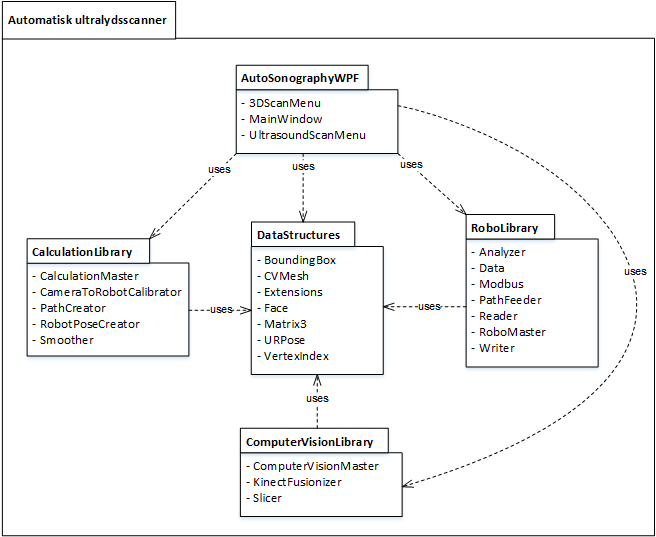
\includegraphics[width=0.9\textwidth]{figurer/d/Design/Pakkediagram}
    \caption{Pakkediagram for Automatisk Ultralydsscanner}
    \label{Pakkediagram}
\end{figure}
\newpage

\chapter{Systemdesign}\label{Systemdesign}
Der er udarbejdet forskellige diagrammer på baggrund af de specificerede systemkrav.  Diagrammerne har til formål at dele systemet op i realiserbare dele for at vise designet af systemet. 

\section{Pakkediagram}
Pakkediagrammet figur \ref{Pakkediagram} giver en oversigt over afhængighederne i PC Applikation.
For at slippe for cykliske forbindelser blev mange datastrukturer flyttet fra CalculationLibrary, ComputerVisionLibrary og RoboLibrary til DataStructures-biblioteket.
DataStructures indeholder altså kun nogle datastrukturer og nogle extension-metoder til disse. 
For forklaringen af indholdet af de øvrige pakker, se klassediagrammerne for hvert bibliotek.

AutoSocograophyWPF inderholder alt, der hører til Grafisk brugergrænseflade (GUI), herunder de tre menuer, 3DscanMenu, StartMenu og UltrasoundMenu. 

ComputerVisionLibrary indeholder klasser, der har at gøre med 3D billedet og konvetering til et mesh, herunder ComputerVisionMaster, KinectsFusionizer og PLYExporter. 

RoboLibray pakken indeholder klasser som robotarmen skal benytte for at kunne flytte sig, herunder Analyzer, Data, Logic, Modbus, PathCreator, PathFeeder, Reader, RoboMaster, URPose og Writer. 

DataStructures

CalculationLibrary

\begin{figure}[H]
    \centering
    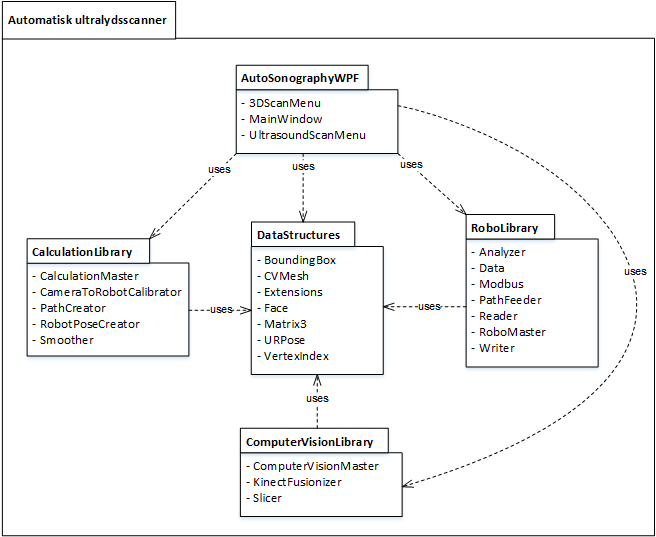
\includegraphics[width=1\textwidth]{figurer/d/Design/Pakkediagram}
    \caption{Pakkediagram for Automatisk Ultralydsscanner}
    \label{Pakkediagram}
\end{figure}
\newpage

\section{Klassediagram}
Dette afsnit beskriver klasserne fra pakkediagrammet. Klassediagrammerne viser strukturen i systemet og deres relationer. Hver klasse indeholder de vigtigste metoder og attributer i klassen, der udgør funktionaliteten i PC Applikation. 

\subsection{GUI}
Denne klasse indeholder brugergrænsefladen af PC Applikation.

\let\labelitemi\labelitemii
\begin{itemize}
\item{MainWindow}\newline
Giver anledning til at foretage et 3D scan. Såfremt en 3D scanning er gennemført giver det også anledning til at starte en ultralydsscanning.
Når menuen startes, oprettes en instans af RoboMaster, for at sætte Robotarm i standard positur. Dette er nødvendigt, hvis Robotarm skulle være i vejen for en 3D scanning.
Hvis der ikke er nogen forbindelse til Robotarm vil der 

\item{3DScanMenu}\newline
I denne menu er der mulighed for at se det nuværende dybdebillede, afgrænse området der skal 3D scannes og foretage en 3D scanning.

\item{UltrasoundScanMenu}\newline
I denne menu kan den procentvise færdiggørelse af ultralydsscanningen følges. Der er også mulighed for at pause samt afbryde ultralydsscanningsprocessen.
\end{itemize}

\begin{figure}[H]
    \centering
    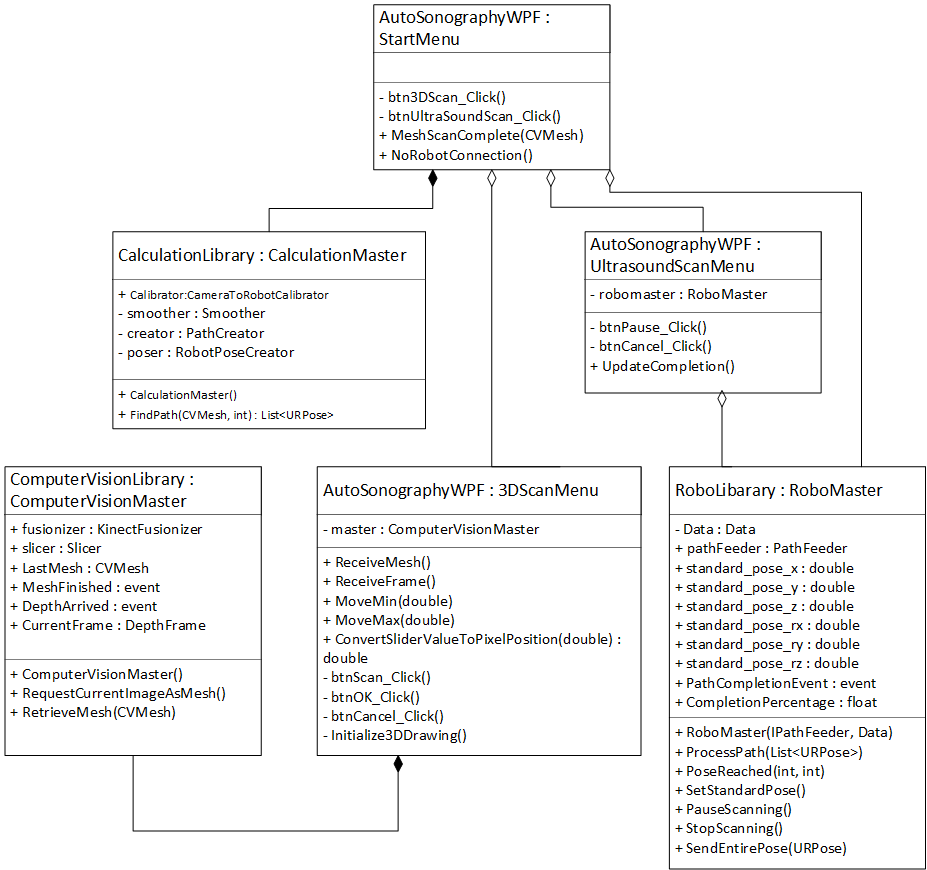
\includegraphics[width=1\textwidth]{figurer/d/Design/Class/uml_class_gui}
    \caption{Klassediagram for GUI}
    \label{class_gui}
\end{figure}
\newpage

\subsection{ComputerVisionLibrary}
Formålet med dette bibliotek er at få en afgrænset 3D scanning fra et 3D kamera.

\begin{itemize}
\item{KinectFusionizeren}\newline
Har til ansvar at åbne Kinect-sensoren, tage det nuværende dybdebillede fra sensoren og konvertere det til en mesh.

\item{ComputerVisionMaster}\newline
Denne klasse virker som den logiske grænseflade til KinectFusionizeren, hvor instansen af den nuværende mesh lagres her.
Andre klasser kan subscribe til ComputerVisionMasteren for at høre hvornår der er en ny mesh tilgængelig.

\item{Slicer}\newline
Denne klasse sørger for at fjerne de punkter i en mesh der er uinteressante:
\begin{enumerate}
\item{Faces der peger nedaf, dvs fejlpunkter. Da 3D kameraet er monteret i loftet, vil den ikke kunne se undersiden af det den skanner.}
\item{Duplikerede punkter. KinectFusionizer outputter punkter der er ens. Disse fjernes af optimeringsårsager.}
\item{Punkter og faces der er uden for det område der ønskes skannet. Dette inkluderer nærtliggende objekter som fx en væg, eller områder på patienten der ikke ønskes skannet.}
\end{enumerate}
\end{itemize}

\begin{figure}[H]
    \centering
    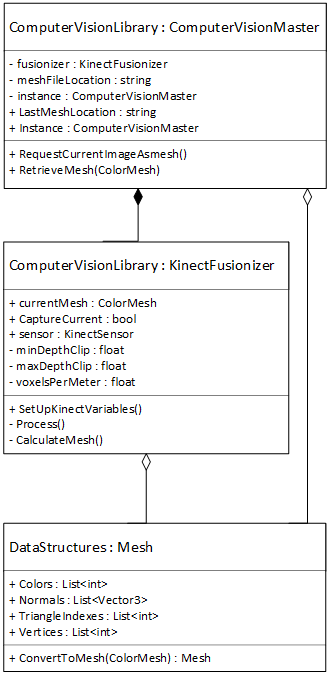
\includegraphics[width=1\textwidth]{figurer/d/Design/Class/uml_class_computervisionlibrary}
    \caption{Klassediagram for ComputerVisionLibrary}
    \label{class_ComputerVisionLib}
\end{figure}
\newpage

\subsection{CalculationLibrary}
Dette bibliotek agerer som bindeledet mellem ComputerVisionLibrary og RoboLibrary.

\begin{itemize}
\item{CameraToRobotCalibrator} \newline
Sørger for at konvertere 3D scanningen givet fra ComputerVisionLibrary fra 3D Kameras rum til Robot Arms rum.
Dette sker ved en kæde af matrix-transformationer i en speciel rækkefølge. 
Normaltvis har man en translation, rotation og skalering, men da Robot Arms og 3D Kameras koordinatsystemer begge er angivet i millimeter, er skaleringen unødvendig.
I tilfældet for dette projekt sker der først en rotering og derefter en translation, for at bestemme transformationsmatricen. 
Hvert punkt i en mesh konverteres så til det nye space. Se bilag \ref{RumTransformation} for inspirationen til denne klasse.

\item{Smoother}\newline
Denne klasse har til ansvar at udjævne en mesh. Med udjævning forstås at 'ensforme' normalerne, altså retningsvektorer i en mesh's faces.
Dette er nødvendigt da 3D Kameras output kan være uperfekt og dermed vil normalerne være ekstreme/deforme. Udjævningen sker gennem laplacian smoothing, se \cite{Smooth} for forklaring af algoritme.

\item{PathCreator}\newline
Klassen afgør listen af punkter i en mesh som der skal findes positurer til Robot Arm ud fra.
For at afgøre stien genereres der en 'bølge' - i implementeringen en squarewave - af punkter der draves over meshen.
De vertices i meshen der tilnærmer sig punkterne i bølgen bedst vil blive udvalgt til stien.

\item{RobotPoseCreator}\newline
I denne klasse vil konverteringen af en mesh-sti til en liste af positurer ske.
For hvert punkt i mesh-stien, vil en vertex' normal findes. 
Ved hjælp af normalen, sti-punktets koordinater samt længden på Robotarms probe kan den forskudte Robot Arm position findes.
Inverteres denne normal, kan det ses som en retningsvektor for en Robotarm.
Retningsvektoren konverteres først til en roll, pitch og yaw - altså roteringer omkring de tre retningsakser; X, Y og Z.
Da man ikke kan afgøre alle tre værdier ud fra en retningsvektor alene, sættes pitch til 0, da det er muligt at 'pege' et vilkårligt sted med en roll-rotering og en yaw-rotering. Disse værdier konverteres herefter til en rotationsvektor.
Positionsvektoren og rotationsvektoren udgør til sammen en positur, som tilføjes til listen af positurer. Matematikken for udregningen af rotationen kan ses på næste side.
\newpage

Givet en tredimensionel retningsvektor med en længde på 1
$$
v_{direction} = (X, Y, Z)
$$
Find de tre rotationer om de tre forskellige akser. Med en retningsvektor alene kan én af disse rotationer ikke findes. Da man vil kunne pege i en vilkårlig retning med en roll-rotering og en yaw-rotering, er pitch sat til 0.
$$ 
roll = acos(Z) \qquad 
pitch = 0 \qquad 
yaw = \begin{cases} 
	-acos(-Y) & X \leq 0\\
	acos(-Y)  & X > 0 \\
\end{cases}
$$

Opstil matricerne der skal bruges for at konvertere roll, pitch og yaw til en rotationsvektor.
%%%%%%%%%%%%%%%%%%%%
% Matricerne 
$$ 
Roll_M = \begin{bmatrix}
    1 & 0 & 0 \\
    0 & cos(roll) & -sin(roll) \\
    0 & sin(roll) & cos(roll)
\end{bmatrix}
\quad
Pitch_M = \begin{bmatrix}
    cos(pitch) & 0 & sin(pitch) \\
    0 & 1 & 0 \\
    -sin(pitch) & 0 & cos(pitch)
\end{bmatrix} 
$$
$$
Yaw_M = \begin{bmatrix}
    cos(yaw) & -sin(yaw) & 0 \\
    sin(yaw) & cos(yaw) & 0 \\
    0 & 0 & 1
\end{bmatrix}
$$ 

Ordnen af rotationerne er vigtig, derfor vil der først foregå en roll rotering, en pitch rotering og til sidst en yaw rotering. Prikken mellem matricerne her er dot-produktet.
$$\mathbb{R} = Yaw_M \cdot Pitch_M \cdot Roll_M $$

Dernæst kan $\theta$ og $\mu$ findes, der bruges til beregningen af $r_x$, $r_y$ samt $r_z$, der samlet udgør den endelige rotationsvektor $v_{rotation}$.

$$\theta = acos\bigg(\frac{\mathbb{R}_{0,0}+\mathbb{R}_{1,1}+\mathbb{R}_{2,2}-1}{2}\bigg) \qquad \mu = \frac{1}{2 \times sin(\theta)}$$

$$r_x =\mu \times(\mathbb{R}_{2,1}-\mathbb{R}_{1,2}) \times\theta $$
$$r_y =\mu \times(\mathbb{R}_{0,2}-\mathbb{R}_{2,0}) \times\theta $$
$$r_z =\mu \times(\mathbb{R}_{1,0}-\mathbb{R}_{0,1}) \times\theta $$
$$v_{rotation} = (r_x, r_y, r_z)$$

\end{itemize}

\begin{figure}[H]
    \centering
    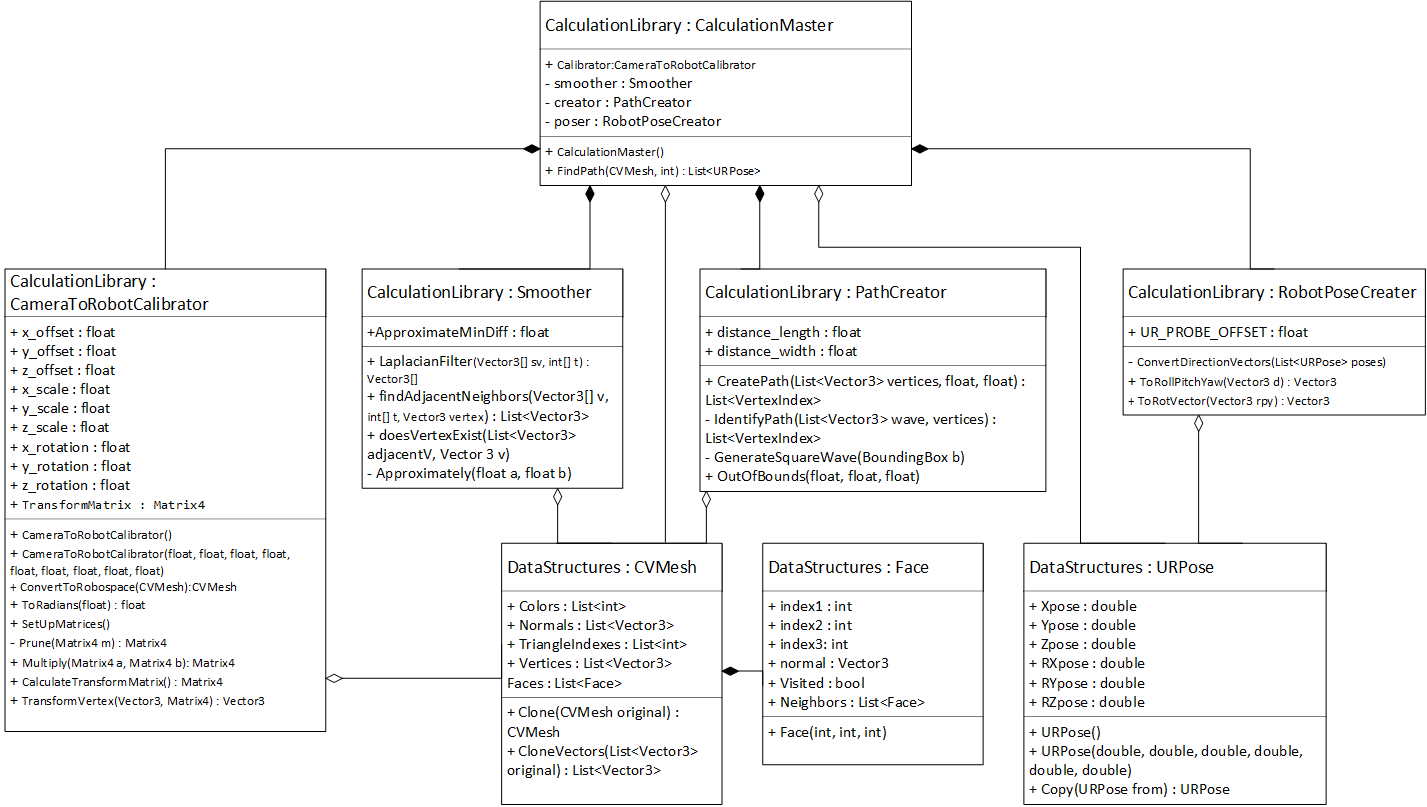
\includegraphics[width=1\textwidth]{figurer/d/Design/Class/uml_class_calculationlibrary}
    \caption{Klassediagram for CalculationLibrary}
    \label{class_ConversionLib}
\end{figure}
\newpage

\subsection{RoboLibrary}
Biblioteket giver mulighed for kommunikation med Robot Arm.

\begin{itemize}
\item{RoboMaster}\newline
Klassen agerer som bindeled mellem de øvrige klasser i biblioteket og GUI.

\item{PathFeeder} \newline
Står for at gennemløbe hver positur i listen, og kommunikere med Data for at finde ud af hvornår den næste positur skal sendes til Robot Arm.

\item{Data}\newline
Klassen virker som en grænseflade mellem den 'logiske' del af biblioteket og dens underliggende reader/writer klasser.

\item{Reader}\newline
Denne klasse står for kontinuerligt at læse data fra Robot Arm, for at afgøre dens nuværende positur. 

\item{Analyzer} \newline
Klassen konverterer det indlæste data til en objekt-orienteret model, altså transformation af bytes til Robot Arms nuværende positur.

\item{Writer}\newline
Klassen har til ansvar at omskrive værdier til binær data. Den omskriver både positurer samt konfigurationer.

\item{Modbus}\newline
Denne klasse skriver binær data ud på Robot Arms IP gennem modbus-protokollen.
\end{itemize}

\begin{figure}[H]
    \centering
    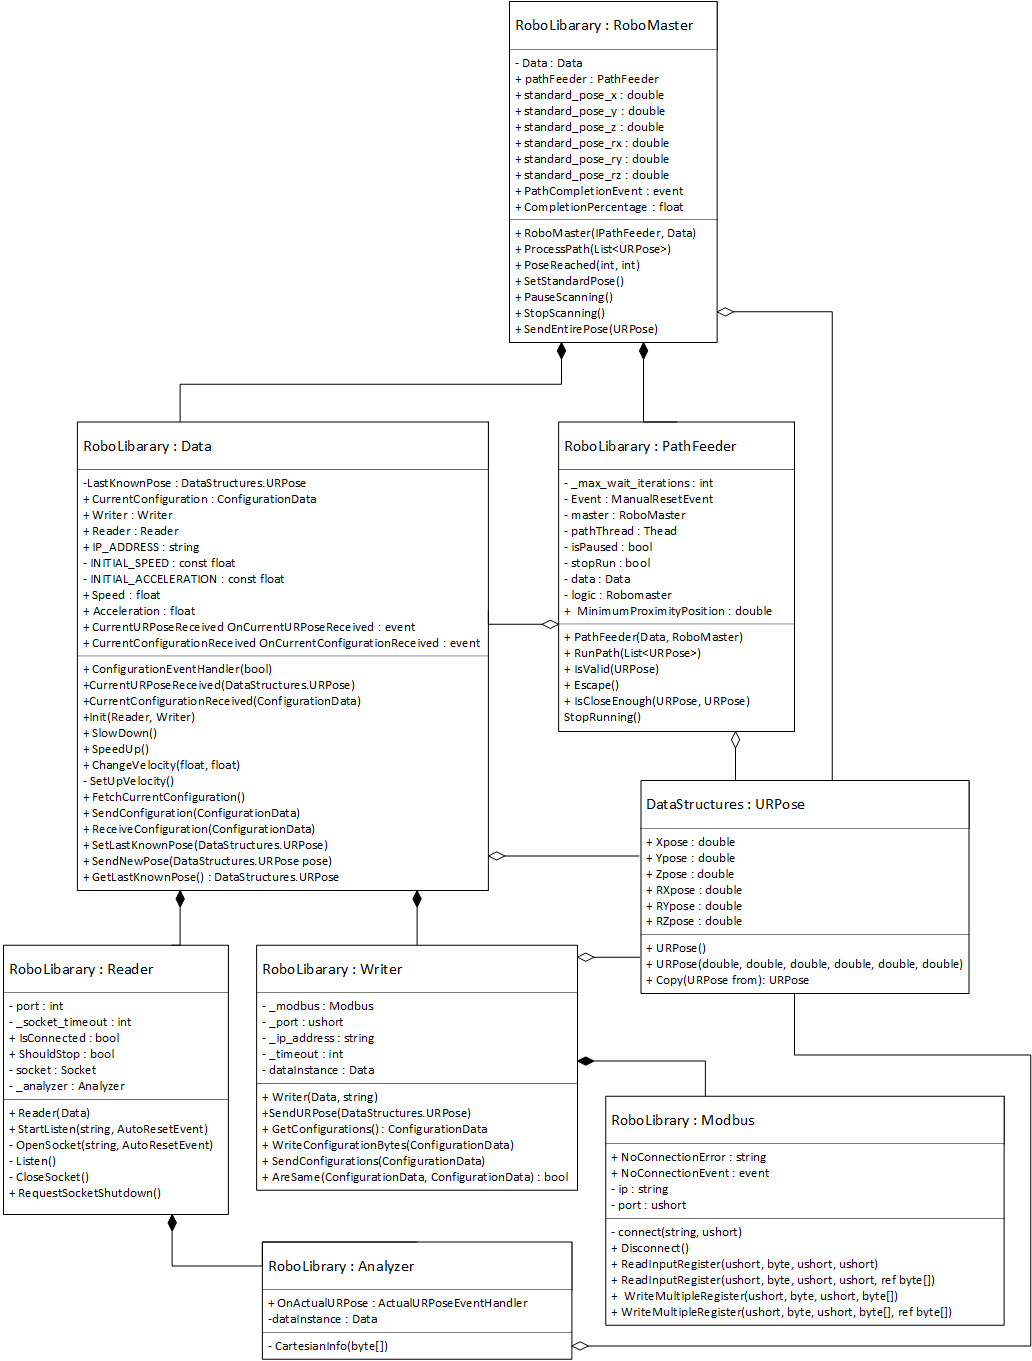
\includegraphics[width=1\textwidth]{figurer/d/Design/Class/uml_class_robolibrary}
    \caption{Klassediagram for RoboLibrary}
    \label{class_RoboLib}
\end{figure}

\newpage
\section{Sekvensdiagrammer}
Der er på baggrund af klassediagrammerne lavet sekvensdiagrammer, som beskriver systemets funktionalitet, og hvor de vigtigse metoder og attributter imellem klasserne er identificeret.

Nedenstående sektioner vil beskrive de vigtigste sekvensdiagrammer i system og fremvise, hvordan klasserne indbyrdes kommunikerer. 

\subsection{Read Robot Data} 
Reader initieres med en IP hvor den skal lytte på. 
Der åbnes en socket på denne IP, og derefter lytter den kontinuert i en baggrundstråd. 
Readeren giver de rå data videre til Analyzer som konverterer dem til Robot Arms nuværende positur.

\begin{figure}[H]
    \centering
    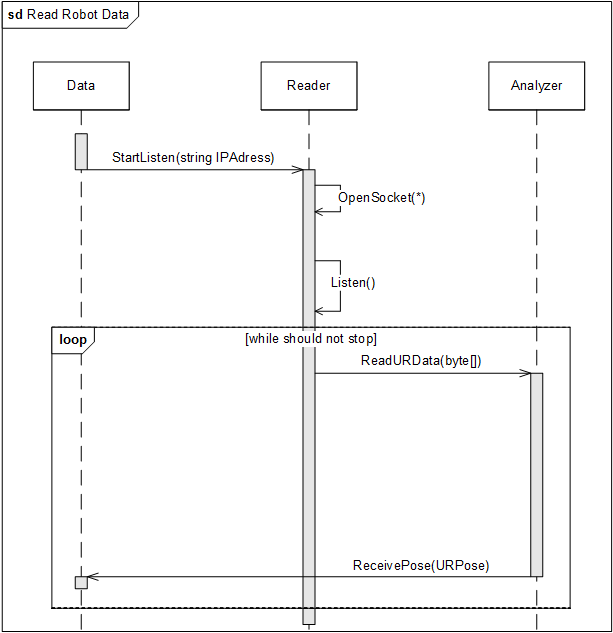
\includegraphics[width=1\textwidth]{figurer/d/Design/Sequence/sd_reading}
    \caption{Sekvensdiagram for Read Robot Data - indlæsning af Robotarms positur}
    \label{sd_reading}
\end{figure}

\subsection{3D scan}
Ved scan vil KinectFusionizeren stå for at tage et dybdebillede fra Kinect-sensoren.
Den vil dernæst konvertere dybdebilledet til en point cloud.Dette trianguleres, så der fås en mesh der efterfølgende kan bearbejdes. 3DScanMenu modtager meshen gennem event-kommunikation.
Gennem de beskræringsparametre der er valgt i menuen vil meshen dernæst beskæres i Slicer, så kun det ønskede område fremkommer. Efter beskæringen vises meshen som en rotérbar 3D model i menuen.

\begin{figure}[H]
    \centering
    \includegraphics[width=1\textwidth]{figurer/d/Design/Sequence/sd_3Dscan}
    \caption{Sekvensdiagram for 3D scan}
    \label{sd_3Dscan}
\end{figure}
\newpage

\subsection{Feed Path}
Efter konvertering af mesh output til robot positur sti, vil listen af positurer sendes fra RoboMaster til PathFeeder. 
Se sekvensdiagrammet 'Path Creation' for en gennemgang af hvordan disse positurer findes.
PathFeeder gennemløber hver positur og sender den næste i listen til Data, som videregiver posituren til Writer.
RoboMaster informeres løbende om hvor langt PathFeeder er med at gennemløbe punkter.
Writer konverterer posituren til binær data, og ModBus skriver dataen ud på Robot Arms register.
Hernæst ser PathFeeder på om Robot Arms nuværende positur har nærmet sig den ønskede positur. 
Når den er tæt nok på, hoppes der ud af 'while'-løkken, og den næste positur kan sendes.
Den Alt der er her skal forstås som at PathFeeder kører i sin egen baggrundstråd der kan pauses. 
Ved terminering af denne baggrundstråd vil PathFeeder stoppe med at videregive nye positurer til Robot Arm.

\begin{figure}[H]
    \centering
    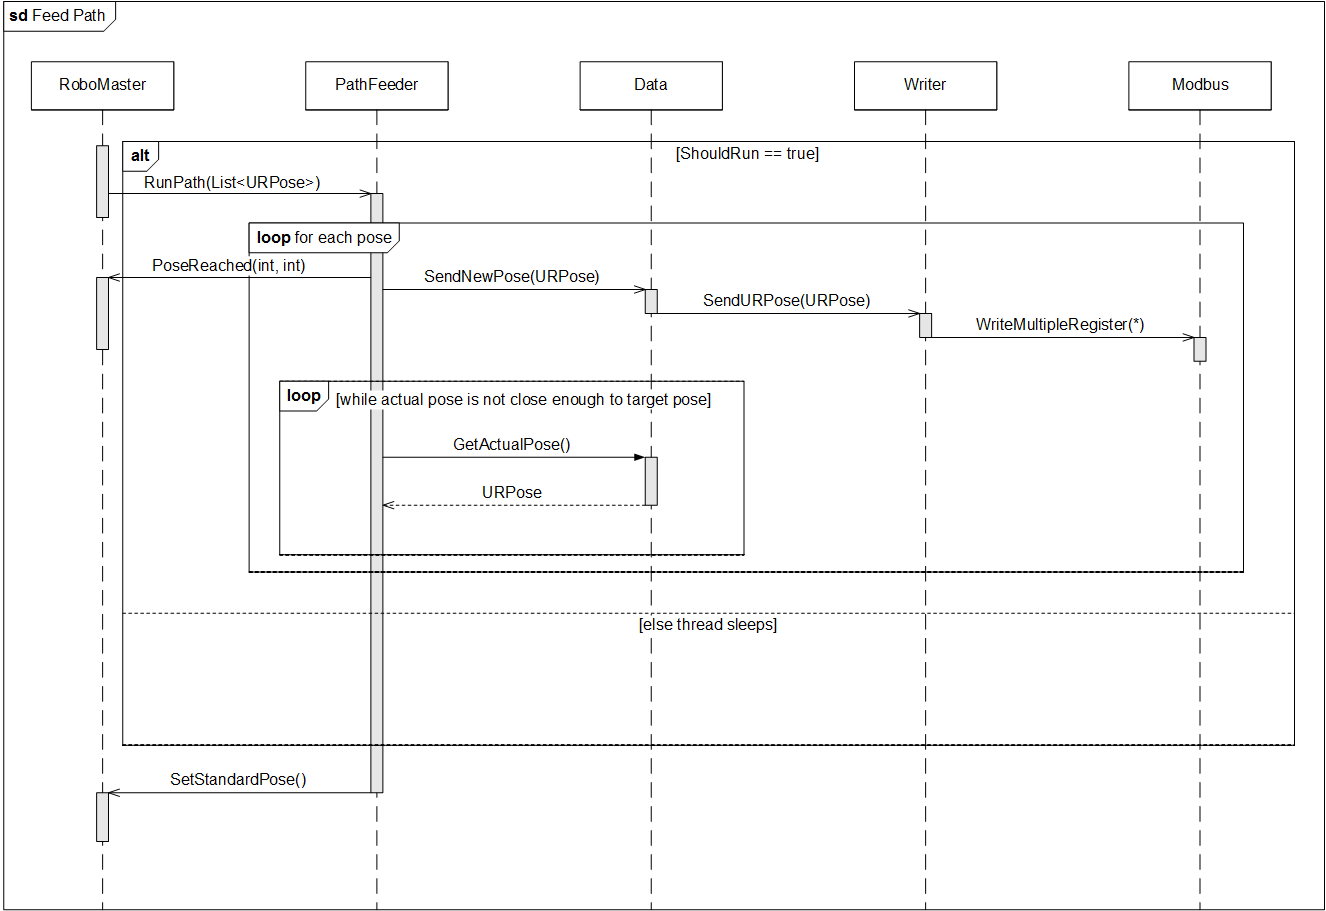
\includegraphics[width=1\textwidth]{figurer/d/Design/Sequence/sd_feedpath}
    \caption{Sekvensdiagram for Feed Path}
    \label{sd_feedpath}
\end{figure}

\subsection{Pathcreation}
Ved tryk på Ultralydsscan-knappen sendes den scannede mesh videre til CalculationMaster. Se sekvensdiagrammet '3D scan' for at se hvordan den scannede mesh opnås.
Først skal meshen konverteres fra 3D Kameras rum til Robot Arms rum, dette sker i CameraToRobotCalibrator, hvor meshen roteres og translateres ift. hvor 3D Kamera befinder sig i virkeligheden.
Efter transformationen skal meshen udjævnes, så de rå og ekstreme normaler i meshen udglattes. Loopet afgør hvor mange gangen meshen skal gennemkøres filteret.
Dernæst sendes den konverterede mesh til PathCreator så der oprettes en liste af de punkter i meshen vi ønsker at Robot Arm skal gennemgå.
Til sidst skal stien der findes i PathCreator konverteres til Robot Arm positurer, da stien i PathCreator kun fortæller position direkte på meshen.
Med denne sti får Robot Arm afdækket overfladen på Patient, hvis den har en Ultralydsscanner monteret.
Stien kan nu videresendes til RoboMaster - se sekvensdiagrammet 'Feed Path' Figur \ref{sd_feedpath}.

\begin{figure}[H]
    \centering
    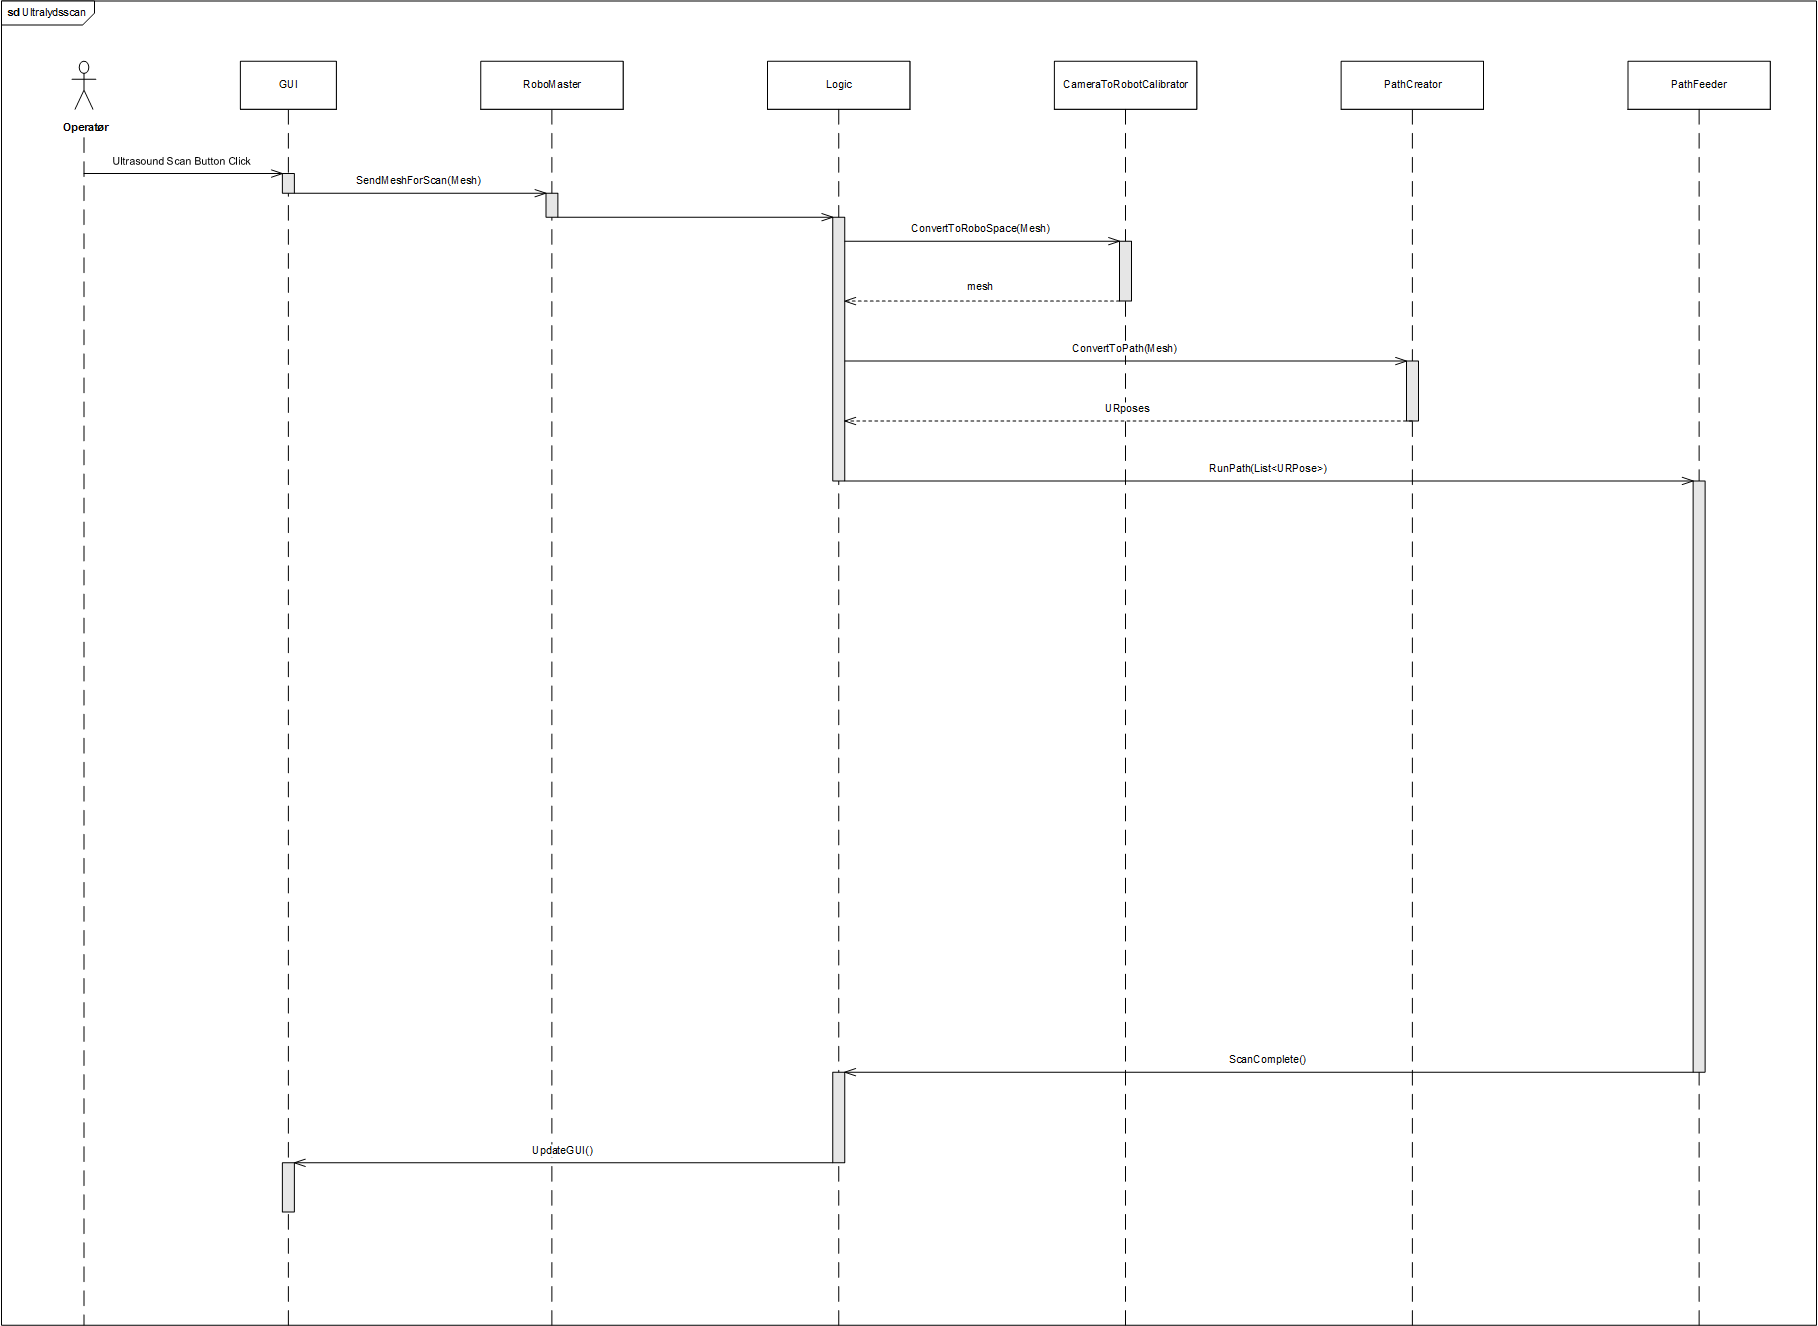
\includegraphics[width=1.4\textwidth, angle =90]{figurer/d/Design/Sequence/sd_ultrascan}
    \caption{Sekvensdiagram for Pathcreation}
    \label{sd_ultrascan}
\end{figure}
\newpage

\section{Detajleret specifikation af klassediagrammer}
Her skal der vises metoderne i hver klasse. 

\section{Tilstandsdiagram}
Dette afsnit beskriver adfærden i systemet ved brug af et tilstandsdiagram. Tilstandsdiagrammet beskriver overgange mellem forskellige tilstande. I UC3: Ultralydsscan brystområde kan Operatør vælge at pause scanningen midlertidig og enten genoptage eller helt stoppe scanning. Figur \ref{stm_Ultra} beskriver Robotarms forskellige tilstande under udførelse af ultralydsscanning. 

\begin{figure}[H]
    \centering
    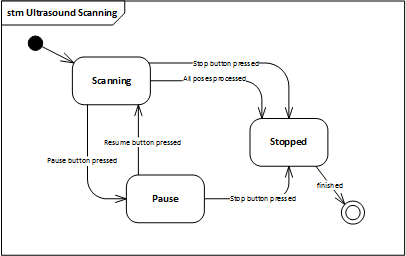
\includegraphics[width=0.7\textwidth]{figurer/d/Design/stm_UC3}
    \caption{Tilstandsdiagram for ultralydsscanning}
    \label{stm_Ultra}
\end{figure}




\chapter{Udviklingsmiljø}\label{Udvikling}
Der er i nedenstående Tabel \ref{Udvikling} opstillet de programmer og versioner der er brugt til udviklingen af Automatisk Ultralydsscanner. 

\begin{table}[htb]
\centering
\begin{tabular}{| l | p{0.20\textwidth}| }
\hline
\textbf{Emne} & \textbf{Version} \\\hline
Windows Education & 10.0.14393 \\\hline
Microsoft Visual Studio Community & 2015 \\\hline
.NET Framework & 4.5.2 \\\hline
JetBrains ReSharper Ultimate & 2016.2.2\\\hline
MeshLab & 1.3.3 \\\hline
Notepad++ & 7.2.1 \\\hline
Unity3D & 5.4.1 \\\hline
Google SketchUp & 16.1 \\\hline
MathCad & 14 \\\hline
Microsoft Kinect API & 1.8 \\\hline
UR10 & 3.1.18024 \\\hline
GitHub & 2016\\\hline
SourceTree & 1.8.3.0 \\\hline

\end{tabular}
\caption{Udviklingsmiljø}
\label{Udvikling}
\end{table}

Til operativsystem (OS) er der anvendt Windows, da .NET-frameworket og Microsoft's Kinect API virker natively på dette OS.

I projektet blev Visual Studio og udviklingsframeworket .NET (i sproget C\#) anvendt til at udvikle PC Applikation. For at beregne code coverage er der anvendt ReSharper.

Til debugging af 3D scanninger er MeshLab og Notepad++ anvendt. 

Google SketchUp er et 3D moduleringsprogam, som i projektet er blevet anvendt til at visualisere de beregninger der skulle til for at rotere Robotarm.

Til 3D visualisering af Automatisk Ultralydsscanner blev Unity anvendt. Dette gjorde det hurtigere at få at overblik over 3D kameras position-offset ift. Robotarm.

Til matematiske beregninger af Robotarms rotation blev Mathcad anvendt.

Til versionsstyring er der brugt GitHub som repository-hosting og SourceTree til git-grænseflade.


\chapter{Test}\label{Test}
I dette afsnit beskrives, hvordan systemet er testet for at sikre, at design og implementeringen lever op til systemkrav, defineret i kravspecifikation bilag \ref{Kravspecifikation}. Der er både udført en accepttest (bilag \ref{Accepttest})  for hele systemet Automatisk Ultralydsscanner og unittest (bilag \ref{Udviklingsdokument} af softwaren i PC Applikation. 

\section{Accepttest}
Accepttesten er lavet for at teste funktionelle og ikke-funktionelle krav, som er beskrevet i kravspecifikation. Testen udføres typisk overfor en kunde, men i bachelorprojektet er accepttesten udførst med vejleder, Michael Alrøe. En godkendt test betyder fejlfri gennemførsel, mens ikke godkendt betyder, at teststeppet ikke kan gennemføres og godkendes. Fejl og årsager er nærmere beskrevet i et andet bilag (HUSK REFERENCE, HVIS DER LAVES ET DOKUMENT!). 

Til accepttesten er der benyttet et testobjekt, udformet som et bryst, som erstatning for patient. For at teste Automatisk Ultralydsscanner bevægelsesmønster, er det valgt at påmontere en ”marker!!!!”, som markerer probens bane over testobjektet. 

\subsection{Funktionelle krav} 
Test af funktionelle krav inkluderer syv forskellige test, da både hovedforløb, udtagelser, og udvidelser i de fire use cases skal testes. Nedenstående tabel viser de forskellige tests, der er udført. 

\begin{table}[htb]
\centering
\begin{tabular}{ | l | p{0.80\textwidth} | }
\hline
\textbf{Testens navn} \\\hline
UC1: Hovedscenarie\\\hline 
UC2: Hovedscenarie \\\hline 
UC2: Undtagelse: Juster 3D billedets skæring \\\hline 
UC3: Hovedscenarie \\\hline 
UC3: Udvidelse: Operatør pauser scanning \\\hline 
UC3: Undtagelse: Operatør stopper scanning \\\hline 
UC4: Hovedscenarie \\\hline 
\end{tabular}
\caption{Test af funktionelle krav} 
\end{table}

Se bilag \ref{Accepttest} Accepttest for det fulde testsetup og resultater af hver test. 

\subsection{Ikke-funktionelle krav} 
De ikke-funktionelle krav er MoSCoW-metoden benyttet til at prioritere kravenes vigtighed. Det er valgt kun at teste ’must’-kravene, som kan ses i nedenstående tabel. 

\begin{table}[htb]
\centering
\begin{tabular}{ | c | p{0.80\textwidth} | }
\hline
\textbf{Type} & \textbf{Navn} \\\hline
Usability & U1. PC Applikation skal have en GUI \\\hline 
Performance & P1. Scanningen med 3D kamera og ultralydsscanning skal max tage 10
minutter til sammen \\\hline 
Performance & P2. Startoptid på PC Applikation skal være max 30 sekunder \\\hline
Performance & P3. 3D kamera skal max bruge 1 minut om at tage 3D billedet \\\hline 
Performance & P4. PC Applikation skal max bruge 1 minut på at færdiggøre brystområdets
positurer til Robotarm \\\hline 
Performance & P5. Ultralydsproben skal bevæges over brystet fra højre mod venstre i en
sinus-lignende kurve \\\hline 
\end{tabular}
\caption{Test af funktionelle krav}
\end{table}

Se bilag Accepttest for det fulde testsetup og resultater for hver test. 

\subsection{Unittest af PC Applikation}
Der er undervejs i udviklingen af PC Applikationen udført unittest af softwarens forskellige dele. 
Testene er lavet i et separat projekt, hvad er code coverage procenten på mm. 

Mere skal skrives herunder. 

Se bilag \ref{Udviklingsdokument} Udviklingsdokument, afsnit 'Test' for en uddybning af de forskellige unittests. 

\subsection{Integrationstest}

\backmatter
\chapter{Bilag}\label{Bilag}

\ref{Satningsliste} Sætningsliste \\
\ref{UR10spec} UR10 Specifikation \\
%\refl{UserManualUR10}


\bibliographystyle{plain}
\bibliography{bibliografi/PRJ3}  % Sætter bibliografien bagerst i dokumentet. Bruger bib-filen PRJ3.

\end{document}